\section{电解质和非电解质}\label{sec:5-1}

\subsection{溶液的导电性}

在上一章,我们已经学习了溶液的一些性质,现在我们来研究一下不同溶质的水溶液的导电性。

\begin{wrapfigure}[10]{r}{7cm}
    \centering
    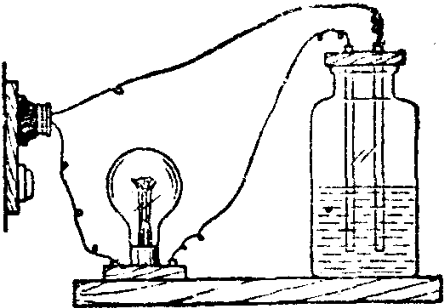
\includegraphics[width=5cm]{../pic/czhx1-ch5-1}
    \caption{试验物质的导电性}\label{fig:5-1}
\end{wrapfigure}

\wrapfiguretrick

\begin{shiyan}
    图 \ref{fig:5-1} 表示的是试验物质导电性的装置,其中主要包括盛有待试验物质的容器、石墨电极和显示电路里有无电流通过的电灯泡等三部分。

    在容器里依次分别加入干燥的食盐晶体、硝酸钾晶体、氢氧化钠晶体、无水硫酸、
    蒸馏水、食盐溶液、硝酸钾溶液、氢氧化钠溶液、硫酸溶液、酒精溶液和蔗糖溶液。
    连接直流电源以后,观察灯泡是不是发光。
\end{shiyan}


从上面的实验可以看到,干燥的食盐晶体、硝酸钾晶体、氢氧化钠晶体、无水硫酸都不导电,
蒸馏水也不导电\footnote{严格地说,蒸馏水也能导电,只是导电能力非常弱,用上述实验装置不能测出。},
可是,食盐、硝酸钾、氢氧化钠、硫酸的水溶液却能够导电。

食盐、硝酸钾和氢氧化钠,不但它们的水溶液能够导电,而且在熔化状态时也能够导电。
蔗糖和酒精就不同,它们的纯净物或水溶液都不能够导电。

\begin{shiyan}
    取几克硝酸钾晶体(或其它易熔的盐如氯化锌、氯化亚锡等)加入瓷坩埚内,放在三脚架和泥三角上,
    插入电极,加热到硝酸钾晶体熔化。连接直流电源,观察灯泡是不是发光。
\end{shiyan}

从上面的实验可以看到,熔化的硝酸钾能够导电。
凡是在水溶液里或熔化的状态下能够导电的化合物叫做\zhongdian{电解质},
在上述情况下都不能导电的化合物叫做\zhongdian{非电解质}。
例如,食盐、硝酸钾、氢氧化钠、硫酸等都是电解质,蔗糖、酒精等都是非电解质。


\subsection{电解质的电离}

为什么食盐、硝酸钾、氢氧化钠等物质在干燥时不导电,而溶于水或熔化时却能导电呢?
为了解决这个问题,必须对这些物质的结构和它们在熔化或溶解的条件下发生的变化进行分析。
我们知道,电流是由带电微粒按一定方向移动而形成的。
例如,金属能够导电,就是由于金属中存在能够自由移动的、带负电的电子。
电解质的水溶液(或熔化而成的液体)既然能够导电,那么,
在这些溶液(或熔化而成的液体)里,是不是也存在着能够自由移动的、带电的微粒呢?
如果有微粒存在,是哪种微粒呢?它们又是怎样形成的呢?下面我们以食盐为例来说明。

我们已经知道,在食盐的晶体里含有带正电的钠离子(\ce{Na+})和带负电的氯离子(\ce{Cl-}),
由于静电的作用,它们既互相吸引,又互相排斥,按一定规则紧密地排列着,
这些离子不能自由移动,因而干燥的食盐不能导电。
当食盐在水里溶解时,在水分子的作用下,减弱了钠离子和氯离子之间的吸引力,
使食盐晶体离解成能自由移动的带电的钠离子和氯离子(图 \ref{fig:5-2})\footnote{严格地说,是形成了与水结合着的钠离子和氯离子。}。
当食盐溶液中插入电极,连接直流电源时,带正电的钠离子向阴极移动,带负电的氯离子向阳极移动,因而食盐溶液就能够导电。

\begin{figure}[htbp]
    \centering
    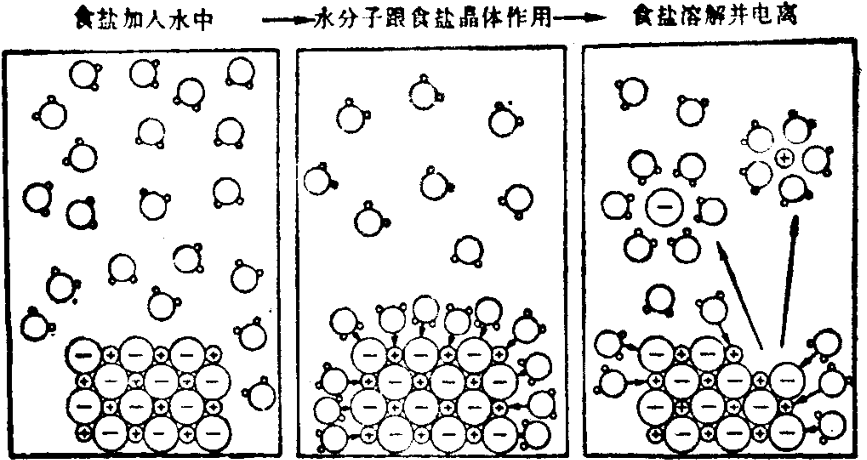
\includegraphics[width=12cm]{../pic/czhx1-ch5-2}
    \caption{食盐在水里的溶解和电离}\label{fig:5-2}
\end{figure}


食盐晶体受热熔化时,由于离子的运动随温度升高而加快,克服了带不同电荷的离子间的引力,
产生了能自由移动的钠离子和氯离子,因而食盐在熔化状态也能导电。

\zhongdian{电解质溶解于水或受热熔化时,离解成自由移动的离子的过程,叫做电离。}

电解质的电离可用如下的电离方程式来表示:
\begin{fangchengshi}
    \begin{aligned}
        & \ce{ \underset{\text{氯化钠}}{\ce{NaCl}} = Na+ + Cl- } \\
        & \ce{ \underset{\text{氢氧化钠}}{\ce{NaOH}} = Na+ + OH- } \\
        & \ce{ \underset{\text{硫酸}}{\ce{H2SO4}} = 2H+ + SO4^{2-} } \\
    \end{aligned}
\end{fangchengshi}

氢氧根离子(\ce{OH-})、硫酸根离子(\ce{SO4^{2-}})都是带电的原子团。
可见,离子不但是带正电或负电的原子,而且也可能是带正电或负电的原子团。

离子所带电荷一般可以根据它们在化合物中的化合价来判断。
例如,金属原子容易失去电子,化合价都是正的,金属离子都带正电,
它的化合价等于几,就可以判断,它带几个正电荷。

电解质溶液里,所有阳离子带的正电荷总数和所有阴离子带的负电荷总数是相等的,
所以整个溶液不显电性。


\begin{xiti}

\xiaoti{为什么用湿手接触正在通电的电器设备更容易发生触电事故?}

\xiaoti{金属能够导电,它们是不是电解质?食盐晶体不能导电,它是不是非电解质?为什么?}

\xiaoti{有人说:“电解质通过电流的时候发生电离”,这句话对吗?为什么?}

\xiaoti{硫酸铜、硝酸钾、硫酸钠、氢氧化钙都是电解质,写出它们在水溶液里的电离方程式。}

\end{xiti}

